%        File: pnas1.tex
%     Created: Wed Apr 30 04:00 pm 2014 E
% Last Change: Wed Apr 30 04:00 pm 2014 E
%
\documentclass[a4paper]{report}
\usepackage[hmargin=2cm,vmargin=2cm]{geometry}

\usepackage{graphicx}

\usepackage{amsmath}
\usepackage{amssymb}
\usepackage{mathrsfs}
\usepackage{gensymb}
\usepackage{algorithm2e}
\usepackage{amsthm}

\newtheorem*{mydef}{Definition}

\usepackage{cite}

\usepackage{framed, color}
\usepackage{soul}
\usepackage[colorlinks=false, urlcolor=blue]{hyperref}

\newcommand{\td}[1]{{\color{blu}\hl{TODO: #1}}}

\definecolor{shadecolor}{rgb}{.93,.93,.93}
\definecolor{blu}{rgb}{0,0,1}
\setlength{\parindent}{0cm}
\setlength{\parskip}{4mm plus1mm minus1mm}


\title{Inter-task effects lead to an unexpected bias in human computation}
\author{Edward Newell, Derek Ruths}

\parindent0pt \parskip8pt

\begin{document}
\maketitle
\section*{Abstract}
\section*{Significance Statement}
\section*{Introduction}

Microtask crowdsourcing platforms like Amazon Mechanical Turk (AMT) make it 
possible to submit batches of small tasks to a large pool of human workers, 
who do the tasks for fun, a sense of purpose, and remuneration 
\cite{kazai2013analysis, Antin20122925}.  
Originally used to distribute clerical work, these platforms 
increasingly serve as a cheap and fast means to engage experimental 
participants and manually annotate datasets in a research 
setting \cite{snow2008cheap}.  
Tasks involving qualitative
judgment (e.g. flagging inappropriate images), natural language annotation,
and object recognition are commonplace, since it is difficult to achieve 
comparable performance using only computers \cite{yuen2011survey}.
%Generally the worker is first given some orientation to the task, and then 
%performs the task repeatedly (e.g. label several images, one after 
%the other).

Such platforms render human cognition into a fluid resource: it is available 
on demand in small units, with low transaction 
cost, from anywhere via the 
Internet\footnote{\href{http://mturk.com}{http://mturk.com}}.
The task requester can 
interact with the platform like a compute server, seamlessly 
integrating human and machine computation.  Researchers have put forward the 
term HPU (Human co-Processing Unit)\footnote{We acknowledge the irony of this 
term: the original meaning of `computer' was a person who performs 
computations, its reference to machines being a personification brought into 
usage in the late 1800s\cite{Dictionary:hl}.}, viewing the introduction of 
microtask platforms as a fundamentally new computing architecture
\cite{5543192}.  

Here, we highlight an important way in which HPUs differ from CPUs, with 
serious implications for the design of tasks.  It is well known that people 
are subject to priming effects 
\cite{BJOP:BJOP1796, No2007, beller1971priming} and, in particular, task-repetition effects
\cite{Gass1999549, sohn2001task}.  
We investigate the effects that the content of earlier tasks has on workers'
outputs in later tasks.  We call such effects 
\textit{inter-task priming}.  Inter-task priming would amount to a kind of
\textit{hysteresis}, meaning that HPU output is not only a function of the 
current input, but also of the history of inputs.

This work supplements the existing research into the factors that affect HPU 
output.  Studies have shown that 
there is a great deal of variance in worker attention and 
accuracy \cite{kazai2013analysis}.
Factors that affect the quality of HPU 
output include level of pay\cite{kazai2013analysis}, 
training\cite{le2010ensuring}, pre-screening 
workers\cite{paolacci2010running}, and user-interface design
\cite{Finnerty2013}.  Research has also investigated \textit{framing}, 
by disclosing to the worker the role of
their task in a larger workflow context \cite{Kinnaird2012281}, 
or describing a meaningful ultimate purpose of the project in which their
task is a part \cite{chandler2013breaking}.  However, to our knowledge, no
study has investigated the effects of inter-task priming.

To characterize such effects, we present a novel  
\textit{algorithmic definition of priming}, and a corresponding method for
measuring priming effects using machine learning algorithms.  
Traditional methods for detecting priming are of limited use in characterizing 
HPU hysteresis, because they are task-specific, and assume that priming results
in a specific class of effects.
Our approach can be applied to any task output, and does not rely on prior 
assumptions about the particular effects brought about by priming.  This 
enables the detection of priming even when the nature of the effects is not 
understood.

In the present work, we investigate inter-task priming for an image-labeling 
task
on the AMT platform.  Each worker is required to label ten images featuring 
food and culture.  We regard these images as being made up of an 
\textit{initial} and \textit{final set}, but, crucially, there is no
distinction made between these sets, nor any interruption in the flow of tasks 
from the view of the worker.
The final image set is always the same, but we randomly assign one of three 
initial sets, and analyze the effect this assignment has on labels attributed 
to the final set.  We employ our novel method for detecting priming effects, as
well as measuring effects on the content and specificity of attributed labels. 

As a point of comparison, we also subject some groups of workers to a kind of
\textit{framing}: we disclose a fictitious, semantically loaded name for the 
task-requester.  The names are chosen to suggest the requester's interest in a 
specific aspect of the image content.  One might reasonably expect that this 
would orient workers to provide a greater quantity and specificity of labels 
which relate to this ``preferred'' content.

Surprisingly, inter-task effects on label orientation and specificity are 
much stronger than those brought about by framing tasks with a funder name. 
Our results 
show that initial tasks can introduce significant bias in subsequent worker 
labeling.  On the other hand, we find evidence that a well-chosen progression 
of tasks could tune workers to produce labels of greater (or lesser) 
specificity.  This suggests that careful consideration should be given to
the progression of tasks when designing a study using a microtask platform.

Even when we are unable to detect priming in the form of a direct
influence on label orientation or specificity, our novel measurement approach 
clearly detects priming. This demonstrates a remarkable feature of the 
approach, whereby priming effects can be quantified without knowing the nature 
of said effects. 

\subsection*{An algorithmic definition of priming}

In psychology, the effects of priming are usually measured in terms of a 
change in the  
speed or accuracy of responses in a task, or in the ability to recognize a 
stimulus object (e.g. a spoken word or an image) when the object is noisier, 
fainter, or briefer [***].  Methods are also employed to measure processes
in the brain of the participant, such as by fMRI.  These approaches are 
well-suited to studying the underlying psychological mechanisms at work.

Our purpose is different: we are interested in assessing the ramifications
that priming of HPUs could have on the applications to which they are employed.
This influences the approach we take to measurement in two ways.  First, we 
switch from focusing on the internal mechanisms of HPUs to focusing strictly 
on the HPU outputs.  Second, we cannot \textit{a priori} know the 
application for which HPUs are being employed, but we would like to measure 
any effects that could in principle impact the application.  These 
considerations motivate us to define priming effects in terms of the 
algorithmic distinguishability of primed output.

One difficulty in constructing a definition of priming is that there would 
appear to be no defensible notion of a ``neutral'' or ``unprimed state''.  A 
participant 
always approaches a task in \textit{some} state of mind.  If no priming 
condition is applied, then the participant is simply primed by her
exposures prior to the experiment, which cannot be known by the experimenter.  
While arguments can surely be made that one treatment or another is 
\textit{more} 
``neutral'', we refrain from proposing a canonical ``null priming treatment''. 
Instead, we define priming relatively, and speak of one treatment being 
\textit{differently primed} from another.

A definition of priming must also consider that the effects of priming will
manifest differently depending on the task that participants perform 
subsequent to priming:  two priming treatments that
produce markedly different output for one task might be 
indistinguishable under another task.  Thus, we define priming
with respect to a task.

A final factor to consider is that people will always differ in their initial
knowledge, specific aptitudes, and in many other intrinsic aspects.  Moreover,
priming may not be ``complete'', in the sense that people's experiences before
priming may continue to have residual effects.  Therefore, we define priming 
in relation to populations, which we regard as having stable distributions of
such latent attributes.

To set up the definition, when a population of people $\mathcal{J}$ performs
a task $\mathcal{T}$ thus producing a population of task-outputs $\mathcal{L}$,
we will write $\mathcal{T}(\mathcal{J}) = \mathcal{L}$. We will also write 
$\mathcal{T}(j) = \ell$ to indicate that a single person, $j$, output $\ell$ 
during $\mathcal{T}$.

\vspace{2mm}
\begin{mydef}
	\upshape
	Two mutually exclusive populations of people, $\mathcal{J}$ and 
	$\mathcal{K}$, are uniformly and randomly subsampled from an initial 
	population $\mathcal{P}$, are exposed to (possibly) different priming 
	treatments, and then perform a task $\mathcal{T}$, 
	producing task-outputs $\mathcal{T}(\mathcal{J})$ and 
	$\mathcal{T}(\mathcal{K})$.
	We say that $\mathcal{J}$ and $\mathcal{K}$ 
	\emph{differ in priming by a degree at least $\theta$},
	if there exists an algorithm $\mathcal{A}$ that takes as input 
	$\mathcal{T}(J)$, $\mathcal{T}(K)$, and $\mathcal{T}(p)$,
	where $J \subset \mathcal{J}$, $K \subset \mathcal{K}$, and $p$ is a 
	person chosen with equal probability from either $\mathcal{J}\setminus J$ 
	or $\mathcal{K}\setminus K$, 
	such that $\mathcal{A}$ outputs the set from which $p$ was drawn
	($\mathcal{J}$ or $\mathcal{K}$) with accuracy $\frac{1+\theta}{2}$.  
\end{mydef}

In the language of computer science, $\mathcal{A}$ is a classifier.  Thus,
intuitively, if there exists a classifier that can distinguish populations 
$\mathcal{J}$ and $\mathcal{K}$ based on their outputs, then they are 
differently primed.

We leave the details of $\mathcal{A}$ unrestricted.  This is 
intentional since we want the definition to depend on the inherent 
potential for two populations to be distinguished, rather than on the 
performance of a particular classifier.

A consequence of this choice is that empirical measures of $\theta$ always
represent lower bounds on the theoretical value appearing in the definition.
As a result, a measured $\theta$ that is greater than zero directly 
supports the conclusion that two populations are differently 
primed, up to the statistical significance of the measurement.  However, if 
$\theta$ is not found to be statistically different from zero, one cannot 
directly
conclude that two populations are the same in priming.  The definition
admits the possibility that there exists some other $\mathcal{A}'$ capable of 
generating a measure of $\theta$ statistically greater than zero. 
Interpreting a result
that $\mathcal{A}$ fails to achieve accuracy significantly better than 
chance depends on the capabilities of $\mathcal{A}$ and the state of the art
of classifier algorithm design.

Note that this definition admits special cases that are equivalent to the
traditional psychological definitions of priming.  If one can show by an
experiment that 
speed, accuracy, or the like, are statistically different for two priming 
treatments, then said experiment could itself be run as a classifier.

This definition substitutes one choice for another: given a task
and two priming treatments, the experimenter need not choose specific effects
to look for, but must instead choose a classifier.  This choice is inherently
less restrictive.  Many general purpose classifiers exist that perform
well in diverse applications [***].  The Naive Bayes classifier stands out as 
a suitable first test to quantify the effects of priming,
because it is simple to implement and requires no domain-specific tuning of 
parameters [***].  We adopt this classifier in the present work and 
denote the measured differences in priming as $\theta_\text{NB}$ to distinguish
them from the theoretical value, $\theta$.

\subsection*{Experimental Setup}
\begin{table}[t]
\centering
	\begin{tabular}{ l  l  l }
		\hline                       
		Treatment & Funder & Priming Image Set	\\ 
		\hline                       
		$\textsc{ambg}$ & None & Ambiguous\\
		$\textsc{cult}_{img}$ & None & Cultural\\
		$\textsc{cult}_{fund}$ & Cultural & Cultural\\
		$\textsc{cult}_{fund,img}$ & Cultural & Cultural\\
		$\textsc{ingr}_{img}$ & None & Ingredients\\
		$\textsc{ingr}_{fund}$ & Nutritional & Ingredients\\
		$\textsc{ingr}_{fund, img}$ & Nutritional & Ingredients\\
		\hline  
	\end{tabular}

%\begin{addmargin}[11em]{11em}
%	\vspace{2mm}
%	$^a$\footnotesize{The full funder names used were ``The Glodal Foundation
%		for Cultural Recognition'' and ``The National Foundation for 
%		Nutritional Awareness''.}
%\end{addmargin}

	\caption{Workers were uniformly randomly
		assigned to one of the treatments listed above.}
	\label{table:1}
\end{table}

\begin{figure}
	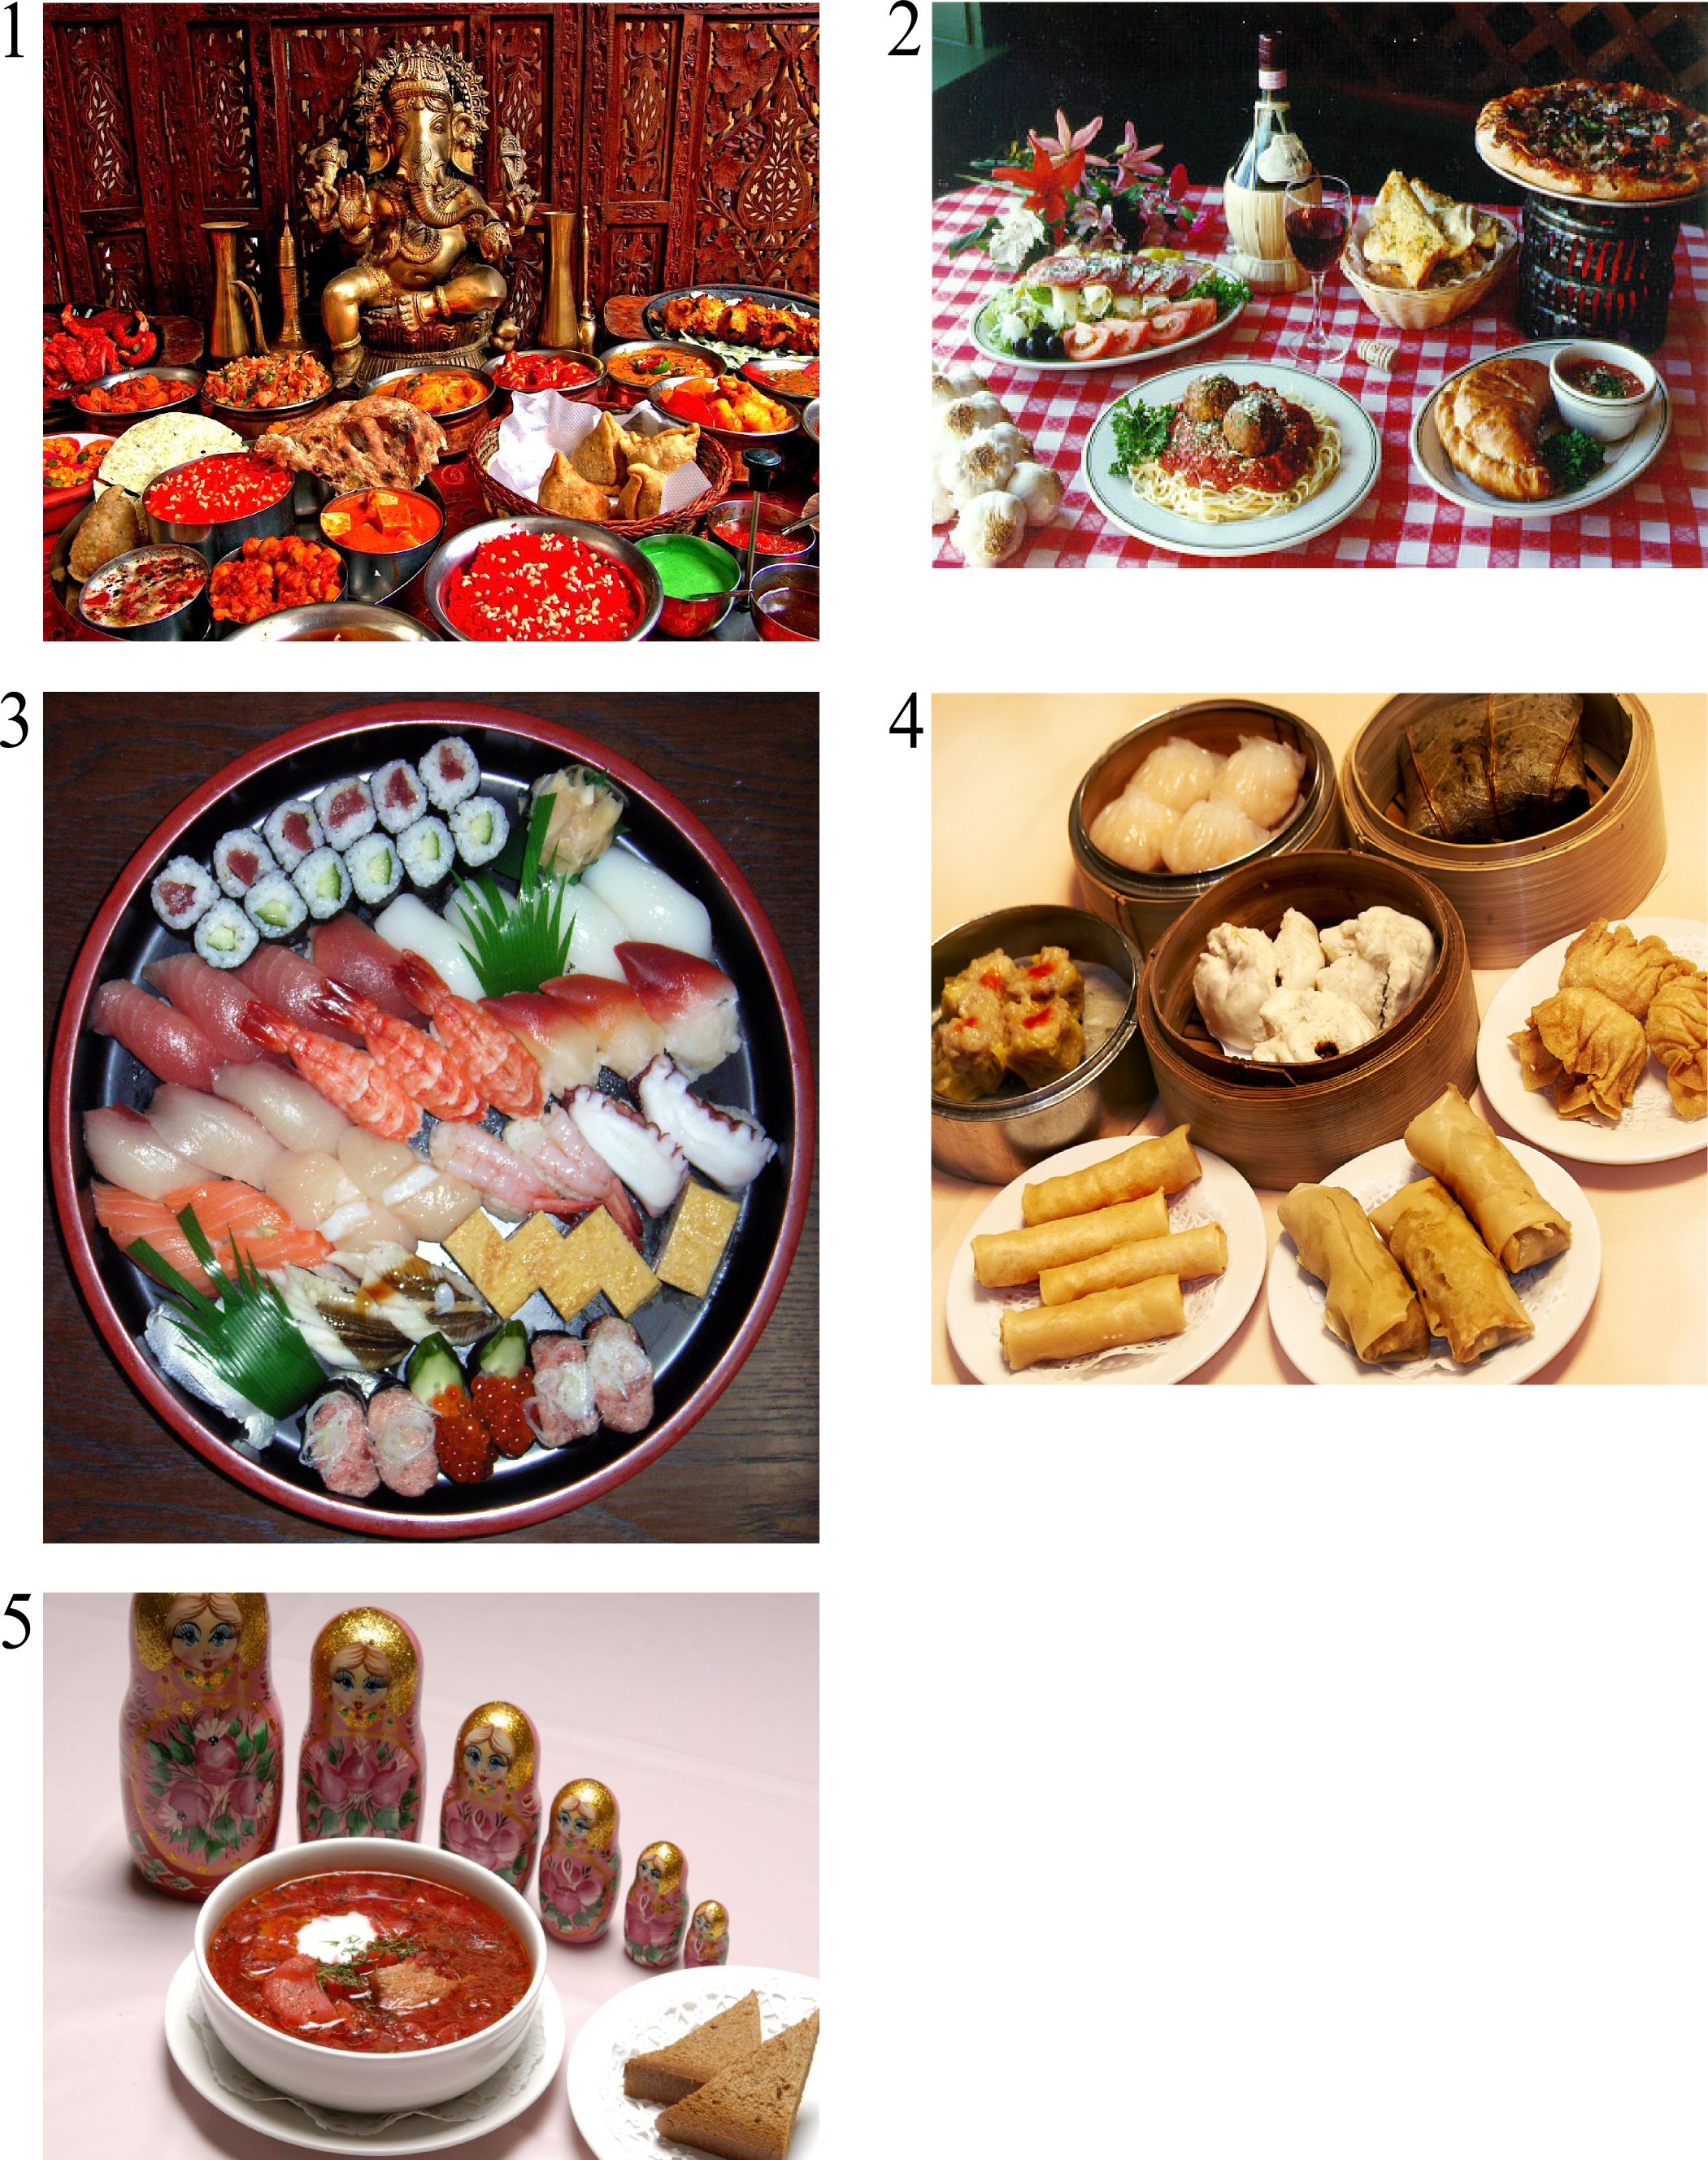
\includegraphics[scale=1.00]{figs/taskImages/testImages.jpg}
	\caption{Testing image set. These images were presented to all workers in 
		the order shown after the priming set of images.}
\end{figure}

\begin{figure}
	\includegraphics[scale=1.00]{figs/taskImages/ambiguous.jpg}
	\caption{ Ambiguous image set. These images were presented to workers from 
		certain treatements (see \textbf{Table 1}) in the order shown.}
\end{figure}

\begin{figure}
	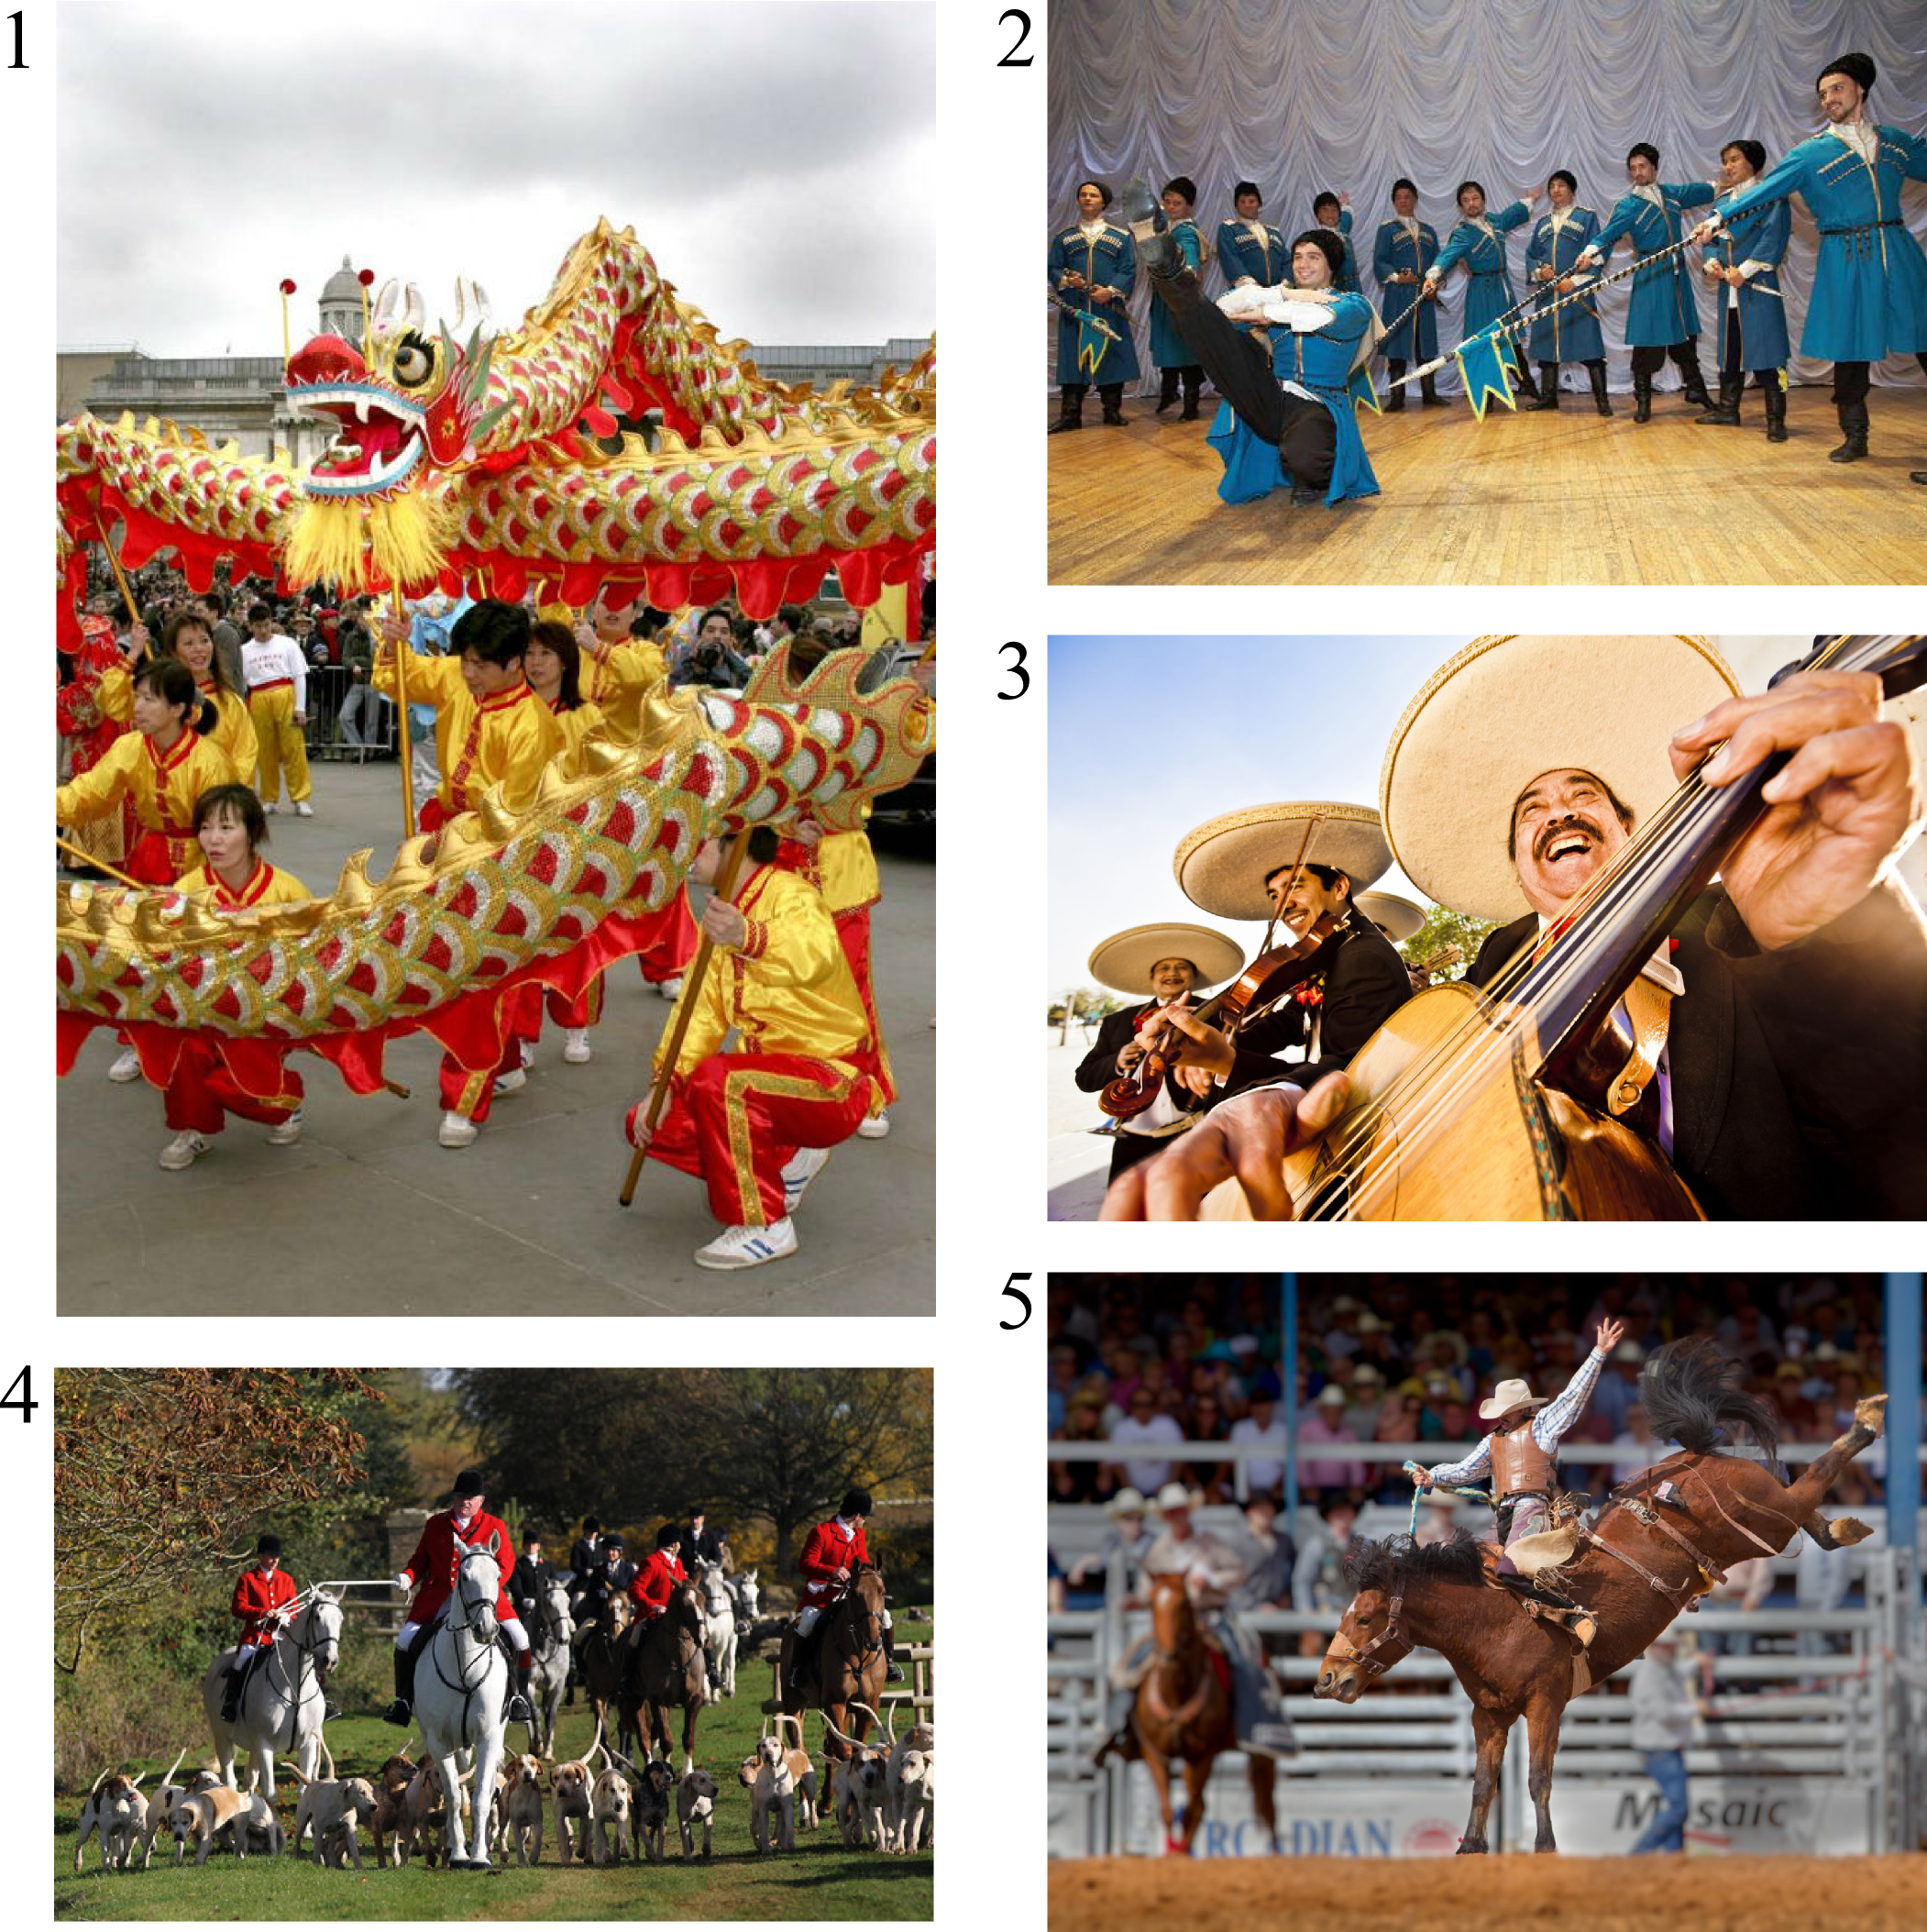
\includegraphics[scale=1.00]{figs/taskImages/cultural.jpg}
	\caption{Cultural image set. These images were presented to workers from 
		certain treatements (see \textbf{Table 1}) in the order shown.}
\end{figure}

\begin{figure}
	\includegraphics[scale=1.00]{figs/taskImages/ingredients.jpg}
	\caption{ Ingredients image set. These images were presented to workers 
		from certain treatements (see \textbf{Table 1}) in the order shown.}
\end{figure}

We solicited 900 AMT workers to perform an image-labeling task relating to
food and culture.  The workers were randomly assigned to one of seven 
treatments shown in \textbf{Table 1}.  Workers were first shown brief 
instructions.  Depending on their treatment, workers were then shown the 
name of a research funder, or this step was skipped.  When shown, 
the funder name was either
``The Global Foundation for Cultural Recognition'', or 
``The National Foundation for Nutritional Awareness''.  Next, workers were
shown ten images, one at a time, and were required to label each image with
five descriptive labels.  For the purpose of analysis, we divide the images
into the \textit{initial} and \textit{final} sets, which are respectively the 
first five and last five images shown.  However, from the perspective of the 
worker, there was no 
distinction or interruption between the initial and final sets. 
The initial set was chosen from one of three sets, depending on the 
treatment, while the final set was always the same.

For the final image set we chose 
images that contain prepared meals and feature a prominent, identifiable 
culture (see \textbf{Fig. 1}).  We intended that the content of these images 
would elicit labels focusing food or culture (or both).
One of the initial image sets, which we call \textit{ambiguous}, was chosen to
be very similar to the final image set, in the sense that it consists of
images of prepared meals.  However, the ambiguous image set was chosen such 
that its cultural features are less prominent and more difficult to identify 
(see \textbf{Fig. 2}).  
The \textit{cultural} initial set features iconic cultural scenes, but no food 
at all (see \textbf{Fig. 3}).  Finally, images from
the \textit{ingredients} initial image set depict separated ingredients, but, 
like the ambiguous set, were chosen to avoid prominent cultural features (see 
\textbf{Fig. 4}).  See the \textbf{Materials and Methods} section for further 
details.

\subsection*{Results}
\paragraph{Earlier tasks and framing both prime workers.}
We tested for priming effects using our definition proposed in the 
introduction, implemented with a Naive Bayes classifier.  
The classifier distinguished the various treatments from one another (pairwise)
with high accuracy, confirming that both priming modalities 
(inter-task and framing) were effective (\textbf{Fig. 5}).  Remarkably, the 
classifier not only 
distinguished treatments tending toward ``different orientations'' 
(e.g. $\textsc{cult}_{img}$ and $\textsc{ingr}_{img}$; \textbf{Fig. 5A}), 
it also distinguished treatments that one might expect would have similar
effects.  For example the greatest accuracy was achieved in 
distinguishing $\textsc{ingr}_{img}$ and $\textsc{ingr}_{fund, img}$, both
of which are primed for a focus on food 
(see \textbf{Fig. 5B}).

\begin{figure}
	\includegraphics[scale=0.94]{figs/f1-thetas_full_pairwise25_img1.pdf}
	\caption{ $F_1$ score and $\theta_\text{NB}$ for the various 
priming treatments, as measured using a Naive Bayes classifier. Each panel 
presents classifier performance results that indicate the difference in
priming between a basis 
treatment, indicated in the inset, and the other treatments, indicated on the
abscissa. }
\end{figure}

Next we looked at the degree to which labels from individual final images 
reveal priming.  It would stand to reason that, as workers proceed through 
the final images, the effects of priming might be ``washed out''.  
Indeed, when labels from just one of the images
in the final set were used, $\theta_\text{NB}$ was lower for later images (see
\textbf{Figure 6}).
Understanding the dynamics of priming wash-out in greater detail is an 
important direction for future work.

\paragraph{Earlier tasks orient focus during later tasks.} 
\begin{figure}
	\includegraphics[scale=0.94]{figs/orientation_specificity.pdf}
	\caption{Percent label composition (culture- vs food-oriented labels) for 
		various images and treatments.  Panel A shows the composition of 
		labels, aggregated over all treatments, as a function of test image.
		Panel B shows the composition of labels, aggregated over all images, as
		a function of treatment.  Panel C shows the composition of labels 
		attributed to the first test image by various treatments.}
\end{figure}

Having demonstrated both inter-task and framing effects, we next
investigated the \textit{nature} of these effects.  To this
end, we constructed an ontology of all the labels attributed to
the final images.   
The ontology is a directed acyclic graph of terms,
with directed edges drawn from abstractions toward instances.  For example,
our ontology contains the path \texttt{food} $\to$ \texttt{ingredients} $\to$ 
\texttt{vegetables} 
$\to$ \texttt{tomato}. We provide more detail about the construction of the 
ontology in the \textbf{Materials and Methods} section.

We counted the number of labels that were of cultural- 
or food-orientation,
based on whether the label had inbound paths from the 
abstract classes \texttt{culture} and/or \texttt{food} in the ontology. Of 
course, food is a central feature of culture, so many labels turned out to be
both culture- and food-oriented in this sense.  Nevertheless, there were many 
food-oriented labels, such as \texttt{bread}, which were culturally highly 
ambiguous, and did not have an inbound path from \texttt{culture} in the 
ontology.  Meanwhile, there were many non-food, culture-oriented labels, such
as \texttt{russian dolls}. 

%The ontology often contained 
%alternative labels for food which were culturally more specific, for example 
%\texttt{roti}, which are attributed cultural-orientation in the ontology.  
%This provided a degree of freedom upon which inter-task priming and framing 
%might act.

Taking the labels from all treatments together, we observed significant 
variance in the label composition (fraction of food- and culture-oriented 
labels) between the various 
images in the final set (see \textbf{Fig. 7A}).  This is to be expected, due 
to differences in the content of the images; for our purpose, we are 
interested in the systematic differences between treatments, not between 
images.

We compared the composition of labels between different treatments by
aggregating labels attributed to all the images from the final set within a 
given treatment (see \textbf{Fig. 7B}).  
Treatments that began by labeling the cultural images, 
subsequently attributed significantly more culture-oriented and fewer 
food-oriented labels to the final images, as compared to the other 
treatments ($\alpha=0.05$).  Meanwhile, all of the $\textsc{ingr}_x$ 
treatments produced more food-oriented labels, but we cannot assert a 
systematic effect at a significance of $\alpha = 0.05$. 

Although the effect on label composition, brought about by having workers 
initially label cultural images, was statistically significant, the effect 
size was admittedly somewhat small (\textbf{Fig 7B}). Since we observed that 
priming 
difference ``wears off'', we analyzed label composition on a per-image basis.
Indeed, for the first image in the final set, workers from 
$\textsc{cult}_{img,x}$ strongly favored culture- over 
food-oriented labels (\textbf{Fig. 7C}). The effect was strong enough to 
essentially invert the proportions of culture- and food-oriented labels 
relative to all other treatments, which favored food-oriented labels.  
This shows that \textit{inter-task effects can dramatically distort the results
of human computation tasks}.

To exhibit the effect longitudinally, as a function of the number of images
labeled since exposure to the initial set, we computed the 
\textit{excess cultural orientation} 
($\Delta_{cult}$) of
$\textsc{cult}_{img}$ relative to $\textsc{ambg}$ as follows: 
\begin{align}
	\Delta_{cult}(i) = \frac{1}{N}\left[ \sum_{w\in\textsc{cult}_{img}} \left(N_{w,cult}^{(i)} - N_{w,food}^{(i)}\right)
	- \sum_{w\in\textsc{ambg}} \left(N_{w,cult}^{(i)} - N_{w,food}^{(i)}\right)\right],
\end{align}
where $N_{w,cult}^{(i)}$ stands for the number of culture-oriented labels 
attributed by worker $w$ to image $i$, while $N_{w,food}^{(i)}$ similarly 
counts food-oriented labels, and $N$ is the total number of labels in a 
treatment.  
Intuitively, this is intended to capture how much 
more culture-oriented the labels from $\textsc{cult}_{img}$ are than those
from $\textsc{ambg}$, for image $i$.

The results from this calculation show the strong influence of the 
initial image set on the labels attributed to the first image in the final set
(see \textbf{Fig. 8}).  However, for later images, the effect immediately 
drops below statistically significant levels, while remaining always positive.

\paragraph{Earlier tasks affect attention to detail during later tasks.} 

Using the ontology described
in the previous section, we compared treatments in their degree of specificity.
When comparing two labels $\ell_1$ and $\ell_2$ produced by different workers,
we say that $\ell_2$ is more specific than $\ell_1$ if there is a 
\textit{directed path} from $\ell_1$ to $\ell_2$.  If there is no directed path
between $\ell_1$ and $\ell_2$, then they are non-comparable.  As an example,
\texttt{tomato} is more specific than \texttt{food}, while \texttt{statue}
and \texttt{food} are non-comparable.

We can compare the specificity of two workers by comparing, for each image,
the labels given by one worker with those of the other.  Thus, we define the
specificity of worker $u$ relative to worker $v$ to be $s(u,v)$:

\begin{align}
	s(u,v) = \sum_{i=1}^5 \;
	\sum_{\ell \in u(i) } \;
	\sum_{m \in v(i)} 
	\left(\mathbf{1}_{[\ell > m]} - \mathbf{1}_{[m>\ell]}\right),
	\label{eq:worker-specificity}
\end{align}
where $u(i)$ denotes the set of labels attributed by worker $u$ to image $i$, 
and $\mathbf{1}_{[\ell > m]}$ evaluates to 1 if $\ell$ is more specific than 
$m$, and 0 otherwise.

We can then define the relative specificity of two treatments, 
$S(\mathcal{U},\mathcal{V})$, to be the average
relative specificity of workers drawn uniformly from the treatments.  
We obtain an estimator, $\hat{S}({\mathcal{U}, \mathcal{V}})$, using the 
sample mean:

\begin{align}
	\hat{S}(\mathcal{U},\mathcal{V}) = 
	\frac{1}{|\mathcal{U} \times \mathcal{V}|}
	\sum_{(u,v) \; \in \; \mathcal{U} \times \mathcal{V}} \;
		s(u,v),
		\label{eq:specificity}
\end{align}

where $\mathcal{U}$ and $\mathcal{V}$ are treatments, formally taken
as sets of workers.

When we compared each of the treatments to \textsc{ambg} in this way, 
all treatments in which a non-ambiguous initial image set was 
displayed have \textit{lower} specificity 
(most, but not all, at $\alpha=0.05$; see \textbf{Fig. 9A}).  To understand
how relative specificity is being attributed, we repeated the calculation of 
specificities relative to \textsc{ambg}, but including only the non-food-, culture-oriented 
labels (see \textbf{Figs. 9D}), and only the non-culture-, food-oriented labels
(see \textbf{Fig. 9G}).  These calculations show that the loss of 
specificity of treatments that initially labeled images other than those from
the ambiguous set, was attributable to specificity of food-oriented labels, 
but not culture-oriented ones.  

It might be the case that labels of a certain semantic connection are less 
influenced by inter-task effects with regard to specificity. Alternatively,
there may have simply been too few cultural labels for an effect on specificity
to manifest (see \textbf{Fig. 7}).
The lower number of cultural labels might be due to the fact that people's 
vocabulary for cultural concepts is less diverse than that for food, or that 
culture, being more abstract, is less ``imageable'' \cite{Swaab200299}.

Nevertheless, the dramatic drop in overall specificity relative to 
\textsc{ambg}, induced when workers begin by labelling the culture or 
ingredients images, demonstrates that 
inter-task effects can strongly influence the specificity of task output.
This is likely to be a major quality factor in nearly all HPU-driven studies.

\td{count the number of occurrences of cultural and food-oriented labels, 
	to see if the non-responsiveness of culture had to do with restricted
number of labels}.



\begin{figure}
	\includegraphics{figs/longitudinal_theta_excess-culture.pdf}
	\caption{Excess culture-oriented label composition in the labels provided
		by $\textsc{cult}_{img}$ as compared to $\textsc{ambg}$, for various
		test images (see \textbf{Eq. 1} for calculation).
	}
\end{figure}


\subsection*{Discussion}

\paragraph{Inter-task effects are strong.}  We expected that by showing
workers the funder names ``The Global Foundation for Cultural Recognition'',
and ``The National Foundation for Nutritional Awareness'', workers would 
be strongly influenced, interpreting this as and indication of what content 
is salient (culture or food).
To our surprise, it turned out that changing the initial set of images that
workers labeled had a much stronger influence on label orientation and 
specificity than did framing the task by naming the funder.
This points to a serious hazard in conducting studies using human computation,
academic or otherwise: even if the requester has 
eliminated surrounding influences to every practical extent, 
\textit{the greatest source of bias might lurk in the tasks themselves}.

Replication of tasks with randomized ordering is one way to abate inter-task
effects.  But the requester could also include an initial set of tasks as a 
``tuning phase''.  During the tuning phase, workers would be primed in a 
controlled way, through exposure to tasks that had been specially picked to
orient worker focus in a useful manner.  Moreover, this phase could double as a
screening phase to select quality workers [***].  However, a deeper 
understanding of the persistence of inter-task effects is needed to know if 
this is viable. 

\paragraph{Subtle priming effects can be detected with $\theta_\text{NB}$.}
The Naive Bayes classifier uses the frequency of occurrence of all labels to
classify workers.  Thus, it incorporates a quite general class of effects which
could be subtle and difficult to anticipate.  This explains why 
$\theta_\text{NB}$ 
between $\textsc{cult}_{fund}$ and $\textsc{ignr}_{img}$ can be comparable with
that between $\textsc{cult}_{fund}$ and $\textsc{cult}_{fund,img}$ 
(see \textbf{Fig. 5}), even though the latter differ much more in label 
orientation and specificity.  Similarly, while the differences in label
orientation between $\textsc{cult}_{img}$ and $\textsc{ingr}_{img}$ drop below 
significance after the first test image (see \textbf{Fig. 8}), 
$\theta_\text{NB}$ remains significant through to the last image.

This demonstrates a powerful feature of the definition of priming in terms of 
algorithmic distinguishability.  Leveraging classifier implementations from
machine learning, one can systematically screen treatments that had allegedly 
been primed differently, against a very large class of potential effects.  This
would allow the analyst to detect that priming had occured without having to 
know anything about what was done to achieve it.

\paragraph{Inter-task similarity drives nuance.}
We observed already that treatments which started by labeling the the 
culture or ingredients image sets had less specificity compared to 
those beginning with the ambiguous image set.  One possible explanation is that
this is a manifestation of \textit{negative priming}.  Negative priming is a 
phenomenon in which a person becomes desensitized to non-salient stimuli to 
which she is repeatedly exposed [***].  Consider that workers who initially 
labeled the ambiguous image set had already seen five images showing 
prepared meals by the time they labeled the first test image.  At that point,
the worker might not regard the labels \texttt{food} or \texttt{meal} to be 
salient, since they do not distinguish the image she is labeling from any of 
the others she had seen already.

We are suggesting that, although workers are not instructed to compare
images in any way, prior tasks nevertheless create a frame of reference
relative to which the content of later tasks are judged.  This in turn 
influences the perception of salience. Thus, in a series of subjective 
characterization tasks that have very similar content, the worker's focus 
will tend to be directed away from generic, shared attributes, towards those 
attributes that are specific and distinguishing.

To support this
claim, we must to assess the perceived similarity between the various 
initial image sets (ambiguous, cultural, and ingredients) and the test set.  
The characterization of image content is deeply complex and has been 
approached from the perspectives of 
art\cite{panofsky1939studies,shatford1986analyzing},
psychology\cite{Tversky1977327}, and information retrieval\cite{Jaimes20002}.  
However, using the labels attributed by workers, we can operationalize
the similarity between two image sets, $X$ and $Y$, as the Jacquard index 
between the sets of labels attributed to them:
\begin{align}
	\text{Sim}(X,Y) = \frac{L(X) \cap L(Y)}{L(X) \cup L(Y)},
\end{align}
where $L(X)$ denotes the set of labels attributed to $X$.  In calculating
the similarity, we used the labels attributed by treatments that were not 
shown a funder name:  \textsc{ambg}, $\textsc{cult}_{img}$, and 
$\textsc{ingr}_{img}$.

Calculated in this way, the ambiguous image set was the most similar to the 
test set, followed by the ingredients set, and the cultural image set
was most different from the test set (see \textbf{Table 2}.)  Comparing
this to the relative specificities calculated for these treatments 
(see \textbf{Fig. 9}) confirms that workers who labeled an initial 
image set that was more similar to the test set attributed more specific 
labels to the test set.

\paragraph{Priming for better HPU performance.}
Thus, if one seeks very nuanced characterizations by human workers, 
our results suggest that the artifacts to be characterized should first 
be sorted into classes that are internally similar. This could be accomplished 
with an iterative approach, which begins with a first, coarse 
characterization of unsorted artifacts. The coarse characterization could then 
be used to sort the artifacts, which could then be served for finer 
characterization.  The sorting and re-characterization could in principle be
repeated several times.

In effect, this creates a hierarchical workflow, where the first, 
coarsely-characterizing HPUs provide a stream of artifacts that is split and 
fed to other HPUs for finer characterization.  This workflow exhibits an 
interesting difference between HPUs and CPUs.  In general,
whenever an aspect of a problem can be parallelized when employing CPUs, one
gains efficiency.  But here, because of HPU hysteresis, we see an example where
one might lose efficiency through parallelization.

\subsection*{Conclusion}
Inter-task priming can have a strong effect.  
For an image-labeling task, inter-task priming was stronger in its effects on 
the orientation and specificity of labels than was the disclosure of 
semantically loaded funder names.  Requesters on microtask platforms should 
beware that strong biases may be introduced do to the particular succession
of tasks they serve to workers.
At the 
same time, inter-task priming might be exploited to improve task output, for 
example, to drive more (or less) nuanced responses.

We demonstrated that our algorithmic definition of priming, and its 
implementation using a Naive Bayes classifier, provides a sensitive,
general-purpose method for detecting priming.  Even when the expected effects 
on label orientation and specificity were slight, $\theta_\text{NB}$ 
was significant.  $\theta_\text{NB}$ provides direct statistical evidence that 
populations have been affected by priming, even when the nature of the 
effects are not understood. 

\subsection*{Materials and Methods}

\textbf{AMT Tasks.} The task described in \textbf{Experimental Setup}
was served to 900 workers, who were uniformly randomly assigned to
treatments.  All treatments had at least 126 task completions.  To obtain 
uniformly sized treatments, we randomly selected 126 samples from each 
treatment. Workers were
only allowed to participate once and could not see the initial or final 
images, nor the funder names when previewing the task.

\textbf{Naive Bayes Classifier.}
The features provided to the Naive Bayes classifier consisted of the labels
that the worker provided along with the image and specific location in which 
the label was entered
(each image had five distinct label inputs).  Thus, \texttt{wine} occurring in 
position 1 of image 2 would be considered as a distinct feature from 
\texttt{wine} occurring in position 2 of image 2. The classifier 
had better performance when this distinction was made.

\textbf{Building the ontology of terms.}  The ontology was built manually
by the experimenters, starting from the corpus of labels. Labels occurring only 
once were discarded.  We created the root classes \texttt{activity}, 
\texttt{adjective}, \texttt{culture}, 
\texttt{food}, and \texttt{thing}. \texttt{culture} and \texttt{food} were 
given top-level status because they were prominently represented in the corpus.
Whenever one label was judged to be a more specific case of another, a
directed edge was drawn from the more general to the more specific. This
judgment call was made by the experimenters.  However, the labels from all 
treatments were aggregated before assembling the ontology,  to 
ensure that the ontology construction would not be affected by 
knowledge of the treatments from which labels originated. 
Labels which were judged to be roughly synonymous were treated as identical,
and labels judged to be misspellings were corrected. 

\textbf{Statistical significance of $\theta_\text{NB}$.}
We test the significance two population's measured $\theta_\text{NB}$ against 
the null hypothesis that that the two populations are in fact identical:
\begin{align}
	\mathbf{H_0}: \theta_\text{NB} = 0 \\
	\mathbf{H_1}: \theta_\text{NB} > 0
\end{align}
If the populations are in fact identical, then the probability that the 
classifier correctly classifies a worker is $\frac{1}{2}$. Let $K$ be a random
variable which denotes the number of correct classifications when the 
classifier is chalenged to classify a total of $n$ workers during 
cross-validation.  Under $\mathbf{H_0}$, the probability distribution of $K$ 
is:
\begin{align}
	\text{Pr}\{K = k | n \} = { n \choose k } \left(\frac{1}{2}\right)^n.
\end{align}
We can reject $\mathbf{H_0}$ at significance $\alpha$ if $\theta_\text{NB}$ 
is greater than a critical value, $\theta_\text{NB}^*$:
\begin{align}
	\theta^*_\text{NB} = \frac{2k^*}{n} - 1
\end{align}
where $k^*$ is the smallest integer in $\{0,\dots,n\}$ that satisfies 
\begin{align}
	\sum_{k \in \{k^*, \dots, n\}} \text{Pr}\{K = k | n \} < \alpha.
\end{align}
For a 5-fold cross-validation with non-overlapping test sets containing 25 
workers ($n = 125$), and a significance of $\alpha = 0.05$, we
have $k^*=73 \implies \theta_\text{NB}^* = 0.168$.






\textbf{Statistical significance of relative specificity.}
We used \textbf{Eq.~\ref{eq:specificity}} to compute the relative specificity
of two treatments.  To analyze relative specificity statistically,
we first develop \textbf{Eq.~\ref{eq:specificity}} from an intermediate 
definition.  Let the specificity of a worker $u$ relative to a 
\textit{basis treatment} $\mathcal{V}$, denoted $S_V(u)$, be the expected 
relative specificity between $u$ and a worker uniformly sampled from 
$\mathcal{V}$:

\begin{align}
	S_V(u) =  \text{E}_V\{s(u,V)\}, \quad V \in_R \mathcal{V},
		\label{eq:basis-specificity}
\end{align}
where $V$ is a random, uniformly sampled worker from $\mathcal{V}$.  We 
subscript the expectation operator with $V$ to indicate 
that the expectation is taken over the distribution of $V$.  Then, the 
relative specificity of two treatments, $S(\mathcal{U},{V})$, can be 
written as:
\begin{align}
	S(\mathcal{U},\mathcal{V}) = 
		\text{E}_U\{S_V(U)\}, \quad U \in_R \mathcal{U},
		\label{eq:treatment-specificity}
\end{align}
where $U$ is a random, uniformly sampled worker from $\mathcal{U}$.  This 
yields 
estimators for $S_V(u)$ and $S(\mathcal{U}, \mathcal{V})$, and their variances
as shown below (note that 
\textbf{Eq.~\ref{eq:treatment-specificity-estimator}} is
equivalent to \textbf{Eq.~\ref{eq:specificity}}):

\begin{align}
	\hat{S}_V(u) &= \frac{1}{|\mathcal{V}|} \sum_{v \in \mathcal{V}} s(u,v), 
		\label{eq:basis-specificity-estimator} \\
		\hat{S}(\mathcal{U},\mathcal{V}) 
		&= \frac{1}{|\mathcal{U}|} \sum_{u \in \mathcal{V}} \hat{S}_V(u),
		\label{eq:treatment-specificity-estimator} \\
		\text{Var}_V\{\hat{S}_V(u)\} 
			&= \frac{1}{|\mathcal{V}|}\text{Var}_V\{s(u,V)\},
		\label{eq:basis-specificity-variance} \\
		\text{Var}_{U,V}\{\hat{S}(\mathcal{U},\mathcal{V})\} 
			&= \frac{1}{|\mathcal{V}|\cdot|\mathcal{U}|^2} 
			\sum_{u\in U}\text{Var}_V\{{s}(u,V)\}.
		\label{eq:treatment-specificity-variance}
\end{align}
\td{There are problems with this.  I'm still trying to figure out how to
	calculate the variance properly.}
$\text{Var}_V\{s(u,V)\}$ can be directly calculated as a sample variance.
\textbf{Equations \ref{eq:basis-specificity-estimator}} through 
\textbf{\ref{eq:treatment-specificity-variance}} provide enough information to test the hypotheses:
\begin{align}
	\begin{matrix}
		\mathbf{H_0}: S(\mathcal{U}, \mathcal{V}) = 0 \\[0.5em]
		\mathbf{H_1}: S(\mathcal{U}, \mathcal{V}) \neq 0
	\end{matrix}
\end{align}

\section*{Acknowledgements}
\section*{References}
\begingroup
\renewcommand{\chapter}[2]{}
\bibliography{newbib.bib}
\endgroup
\bibliographystyle{plain} 

\section*{Figure Legends}

\paragraph{Table 1.}
	Experimental treatments.  Workers were uniformly randomly
	assigned to one of the treatments listed above.  The full funder 
	names used were ``The Global Foundation
	for Cultural Recognition'' and ``The National Foundation for 
	Nutritional Awareness''.  The ambiguous, cultural, and ingredients 
	initial image sets are shown in \textbf{Figs. 2}, \textbf{3}, and 
	\textbf{4}.

\paragraph{Figure 1.}
	Posterior image set. These images were presented to all workers after the 
	initial image set, in the order shown. 

\paragraph{Figure 2.}
	Ambiguous image set. These images were presented to workers from certain
	treatments (see \textbf{Table 1}) as the initial image set, in the order 
	shown.  

\paragraph{Figure 3.}
	Cultural image set. These images were presented to workers from 
	certain treatments (see \textbf{Table 1}) as the initial image set, in the 
	order shown.  

\paragraph{Figure 4.}
	Ingredients image set. These images were presented to workers from 
	certain treatments (see \textbf{Table 1}) as the initial image set, in the 
	order shown.  

\paragraph{Figure 5.}
$F_1$ score and $\theta_\text{NB}$ for the various 
priming treatments, as measured using a Naive Bayes classifier. Dotted lines 
show the 95\% confidence interval
assuming the classifier performed no better than chance.  Each panel 
presents performance results for the binary classification between a basis 
treatment, indicated by the inset, and other treatments, indicated on the 
abscissa.

\paragraph{Figure 6.}
$F_1$ score and $\theta_\text{NB}$ for the classification of 
$\textsc{cult}_{img}$ and $\textsc{ingr}_{img}$ using a Naive Bayes 
classifier.  Dotted lines 
show the 95\% confidence interval
assuming the classifier performed no better than chance.  The classifier is provided only the labels attributed to
particular images as indicated on the abscissa.

\paragraph{Figure 7.}
Percent label composition (culture- vs food-oriented labels) for 
various images and treatments.  Panel A shows the 
composition of labels, aggregated over all treatments, as a function of 
final image.
Panel B shows the composition of labels, aggregated over all images, as
a function of treatment.  Panel C shows the composition of labels 
attributed to the first final image by various treatments.

\paragraph{Figure 8.}
Excess culture-oriented label composition in the labels provided
by $\textsc{cult}_{img}$ as compared to $\textsc{ambg}$, for various
final images (see \textbf{Eq. 1} for calculation).

\paragraph{Figure 9.}
Relative specificity of various treatments.
Each panel shows the comparison between a basis treatment (inset) and 
target treatments (abscissa).
Bar heights indicate relative specificity of the target 
treatment compared to the basis (a positive quantity means the target 
is more specific), and are normalized to units of standard 
deviations of the null comparison.  Dotted horizontal lines indicate
the 95\% confidence interval for the null comparison, which necessarily
has zero relative specificity (see \textbf{Methods} 
for an explanation of the null comparison).  Panels D, E, and F 
represent relative specificity calculated using only culture-oriented
labels, while panels G, H, and I using only food-oriented labels.
Labels that are both culture- and food-oriented are excluded from the
calculations for panels D through I.

\paragraph{Figure S1}
Relative specificity of various treatments, for labels attributed
to the first final image.
Each panel shows the comparison between a basis treatment (inset) and 
target treatments (abscissa).
Bar heights indicate relative specificity of the target 
treatment compared to the basis (a positive quantity means the target 
is more specific), and are normalized to units of standard 
deviations of the null comparison.  Dotted horizontal lines indicate
the 95\% confidence interval for the null comparison, which necessarily
has zero relative specificity (see \textbf{Methods} 
for an explanation of the null comparison).  Panels D, E, and F 
represent relative specificity calculated using only culture-oriented
labels, while panels G, H, and I using only food-oriented labels.
Labels that are both culture- and food-oriented are excluded from the
calculations for panels D through I.

\end{document}


